\clearpage{\pagestyle{empty}\cleardoublepage}

\chapter{\wbx\ analysis: SR cut-flow}\label{app:wbxSR}

In this appendix some more information about the cut-flow in the
signal regions for the \wbx\ analysis is given. We remind in 
Table~\ref{tab:wbxselectionBIS} the signal regions definition.
In the following sections the selected number of events selected in the
electron (Table~\ref{tab:cftabELE}) and muon (Table~\ref{tab:cftabMUON})
channels are reported, and the distribution of the discriminant variable
\mreco\ is shown in the various signal regions.

\begin{table}[h!]
\begin{center}
\begin{tabular}{lll}
\toprule
Selection & Signal Region & Requirements \\
\midrule
Preselection & & One electron or muon  \\
             & & $\met >20\gev$, $\met +m_{\rm T}>60\gev$ \\
             & & $\geq 4$ jets, $\geq 1$ $b$-tagged jets \\
\midrule
\loose\ selection & SR0 & Preselection  \\
                  & SR1 & +\hskip5ex$\geq 1~W_{\rm had}$ candidates \\
                  & SR2 & +\hskip5ex$\HT>800\gev$ \\
                  & SR3 & +\hskip5ex $\pt(b_1) > 160\gev$\\
                  & SR4 & +\hskip5ex$\pt(b_2) >80\gev$ \\
                  & SR5 ($\equiv$\loose) & +\hskip5ex$\Delta R(\ell,\nu)<1.2$ \\
\midrule
\tight\  selection & SR5 & \loose\ selection \\
     	      & SR6 &  +\hskip5ex min$\Delta R(\ell,b)>1.4$\\
              & SR7 ($\equiv$\tight) & +\hskip5ex min$\Delta R(W_{\rm had},b)>1.4$ \\
\bottomrule
\end{tabular}
\caption{Summary of event selection requirements.}
\label{tab:wbxselectionBIS}
\end{center}
\end{table}

\newpage

\section{Event yields in the electron and muon channels}\label{app:wbxSR_yields}


\begin{table}[h!tb]\centering
\resizebox{1.\textwidth}{!}{
        \begin{tabular}{l c c c c } \toprule\toprule
 & $T\bar{T}$ (600) chiral 		 & $t\bar{t}$ MC@NLO 		 & non-$t\bar{t}$ 		 & Data 		 \\ \midrule 
  Preselection  & $189.67 \pm 4.83$  & $92135.41 \pm 189.70$  & $29216.10 \pm 228.75$  & $117565.00 \pm 342.88$ \\ 
 +$\geq 1~W$ candidate  & $88.83 \pm 3.28$  & $2918.44 \pm 33.94$  & $677.93 \pm 31.70$  & $3845.00 \pm 62.01$ \\ 
 +$\HT>800\gev$  & $86.26 \pm 3.25$  & $726.61 \pm 17.78$  & $274.47 \pm 22.04$  & $1109.00 \pm 33.30$ \\ 
 +$\pt(b_1) > 160\gev$  & $74.79 \pm 3.01$  & $355.86 \pm 12.38$  & $153.24 \pm 15.91$  & $560.00 \pm 23.66$ \\ 
 +$\pt(b_2) >80\gev$  & $58.54 \pm 2.68$  & $195.30 \pm 9.08$  & $62.49 \pm 10.83$  & $263.00 \pm 16.22$ \\ 
 +$\Delta R(\ell,\nu)<1.2$  & $49.24 \pm 2.47$  & $119.27 \pm 6.93$  & $25.03 \pm 5.71$  & $164.00 \pm 12.81$ \\ 
 +min$\Delta R(\ell,b)>1.4$  & $38.02 \pm 2.16$  & $10.94 \pm 2.30$  & $11.01 \pm 2.18$  & $27.00 \pm 5.20$ \\ 
 +min$\Delta R(W,b)>1.4$  & $30.49 \pm 1.94$  & $4.34 \pm 1.63$  & $4.25 \pm 1.69$  & $18.00 \pm 4.24$ \\ 
\bottomrule\end{tabular}}
        \caption{
Number of observed events, integrated 
          over the whole mass spectrum, compared to the Standard Model expectation for
          the $e$+jets channel
          in the Signal Regions (see Table~\ref{tab:wbxselectionBIS} for the
        region definitions).
          The expected signal yields for a chiral 
          fourth-generation $\T$ quark with $m_{\T}=600\gev$ are also shown.
          The quoted uncertainties are only statistical.}\label{tab:cftabELE}
\end{table}


\begin{table}[h!tb]\centering
\resizebox{1.\textwidth}{!}{
        \begin{tabular}{l c c c c c } \toprule\toprule
 & $T\bar{T}$ (600) chiral 		 & $t\bar{t}$ 		 & non-$t\bar{t}$ 		 & Tot Bkg 		 & Data 		 \\ \midrule 
  SR0  & $190 \pm 5$  & $109558 \pm 209$  & $36747 \pm 274$  & $146304 \pm 344$  & $144316 \pm 380$ \\ 
 SR1  & $79 \pm 3$  & $3417 \pm 37$  & $757 \pm 33$  & $4174 \pm 50$  & $4556 \pm 67$ \\ 
 SR2  & $75 \pm 3$  & $848 \pm 20$  & $280 \pm 21$  & $1128 \pm 28$  & $1250 \pm 35$ \\ 
 SR3  & $64 \pm 3$  & $456 \pm 14$  & $139 \pm 13$  & $595 \pm 19$  & $663 \pm 26$ \\ 
 SR4  & $48 \pm 2$  & $242 \pm 10$  & $56 \pm 9$  & $297 \pm 13$  & $335 \pm 18$ \\ 
 SR5  & $39 \pm 2$  & $144 \pm 8$  & $25 \pm 4$  & $169 \pm 9$  & $184 \pm 14$ \\ 
 SR6  & $29 \pm 2$  & $16 \pm 3$  & $11 \pm 3$  & $26 \pm 4$  & $34 \pm 6$ \\ 
 SR7  & $23 \pm 2$  & $6 \pm 2$  & $6 \pm 3$  & $12 \pm 3$  & $19 \pm 4$ \\ 
\bottomrule\end{tabular}}
        \caption{Number of observed events, integrated 
          over the whole mass spectrum, compared to the Standard Model expectation for
          the $\mu$+jets channel 
          in the Signal Regions (see Table~\ref{tab:wbxselectionBIS} for the
        region definitions).
          The expected signal yields for a chiral 
          fourth-generation $\T$ quark with $m_{\T}=600\gev$ are also shown.
          The quoted uncertainties are only statistical.}\label{tab:cftabMUON}
\end{table}


\section{Reconstructed mass in the SRs}\label{app:wbxSR_mreco}

Figure~\ref{fig:mrecoSRs} shows the progress of signal selection
and background rejection in the various signal regions that progressively
approach the final \tight\ selection.

\begin{landscape}
\begin{figure}[htb]\begin{center}
\vskip-1cm
	\subfigure[]{\label{fig:mrecoSR1}
  	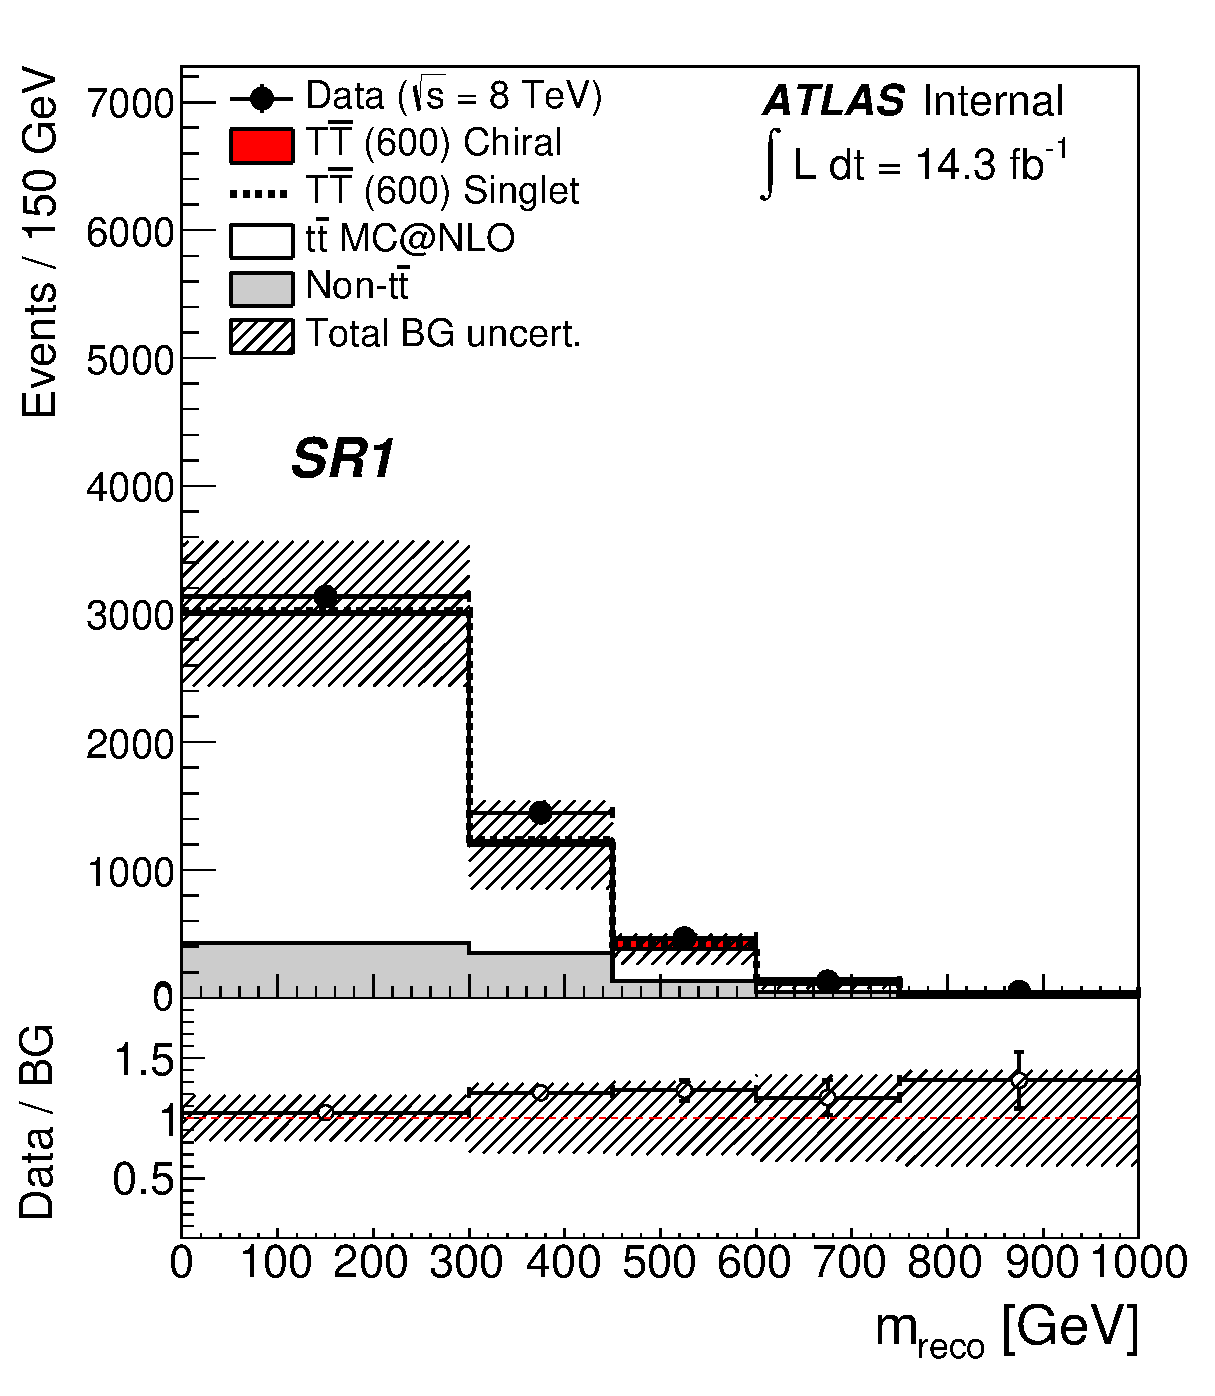
\includegraphics[width=0.37\textwidth]{wbx_analysis_14ifb/figures/THESIS_c6_cutflow/VLQAna_WbX_1W_MWb_4_ELEMUON_cutflow1_NOMINAL.eps}}
	\subfigure[]{\label{fig:mrecoSR2}
  	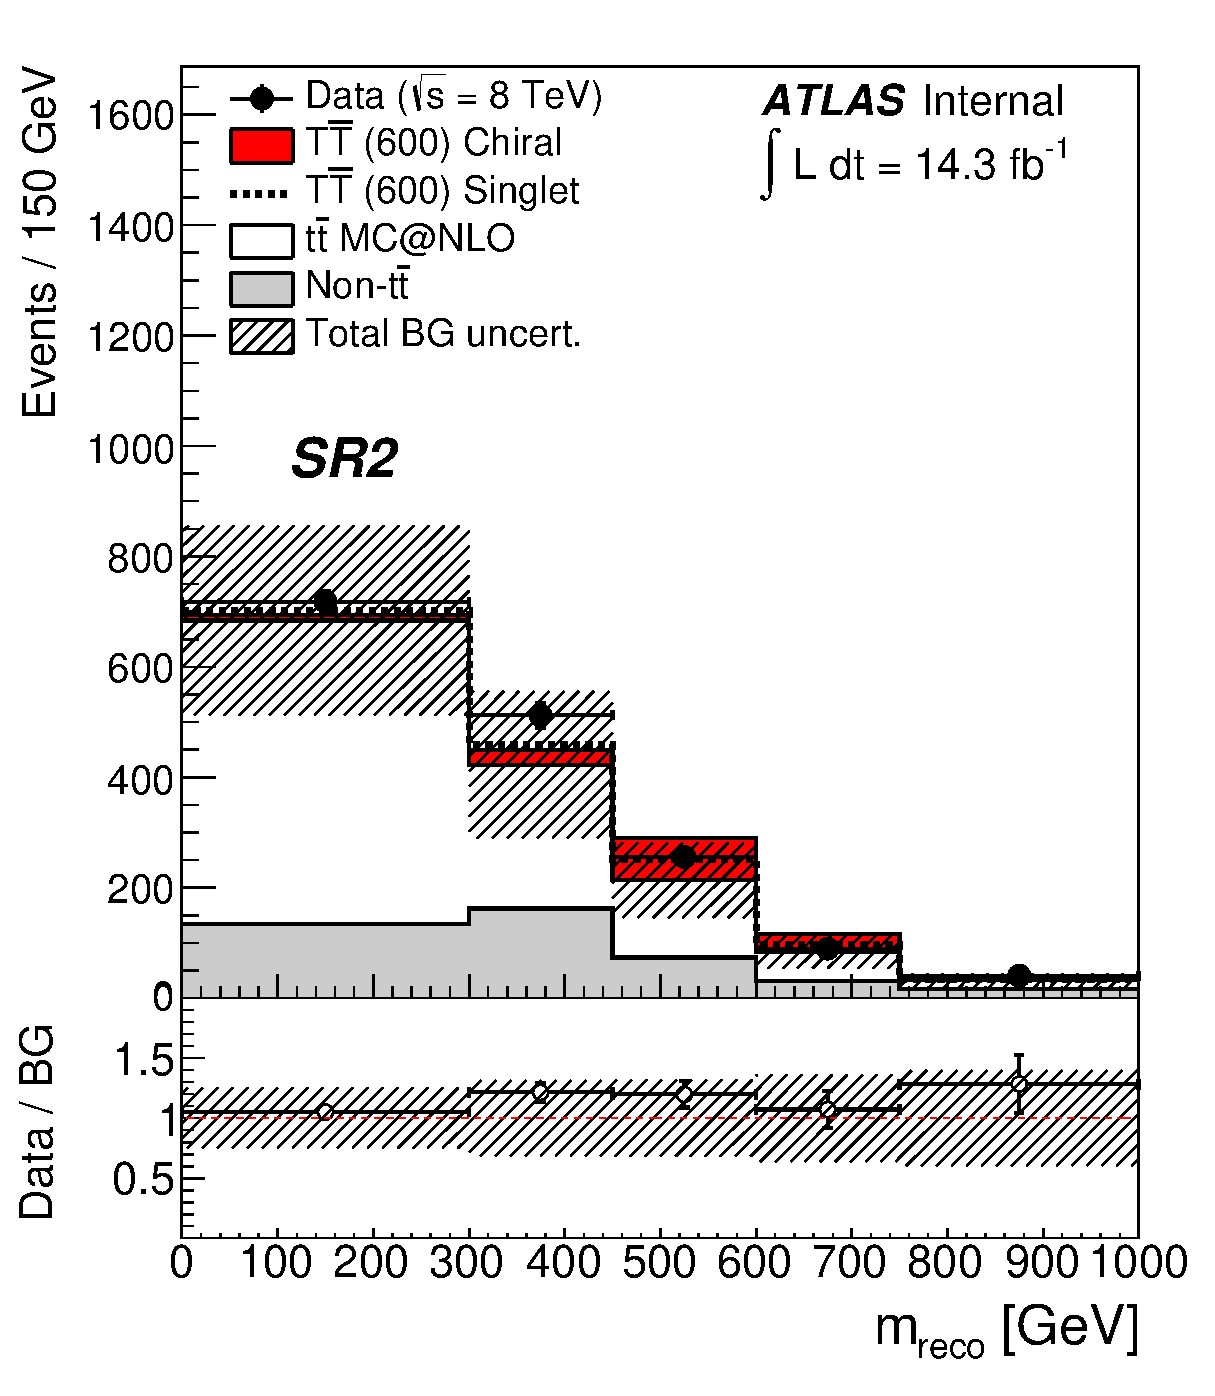
\includegraphics[width=0.37\textwidth]{wbx_analysis_14ifb/figures/THESIS_c6_cutflow/VLQAna_WbX_1W_MWb_4_ELEMUON_cutflow12_NOMINAL.eps}}
	\subfigure[]{\label{fig:mrecoSR3}
  	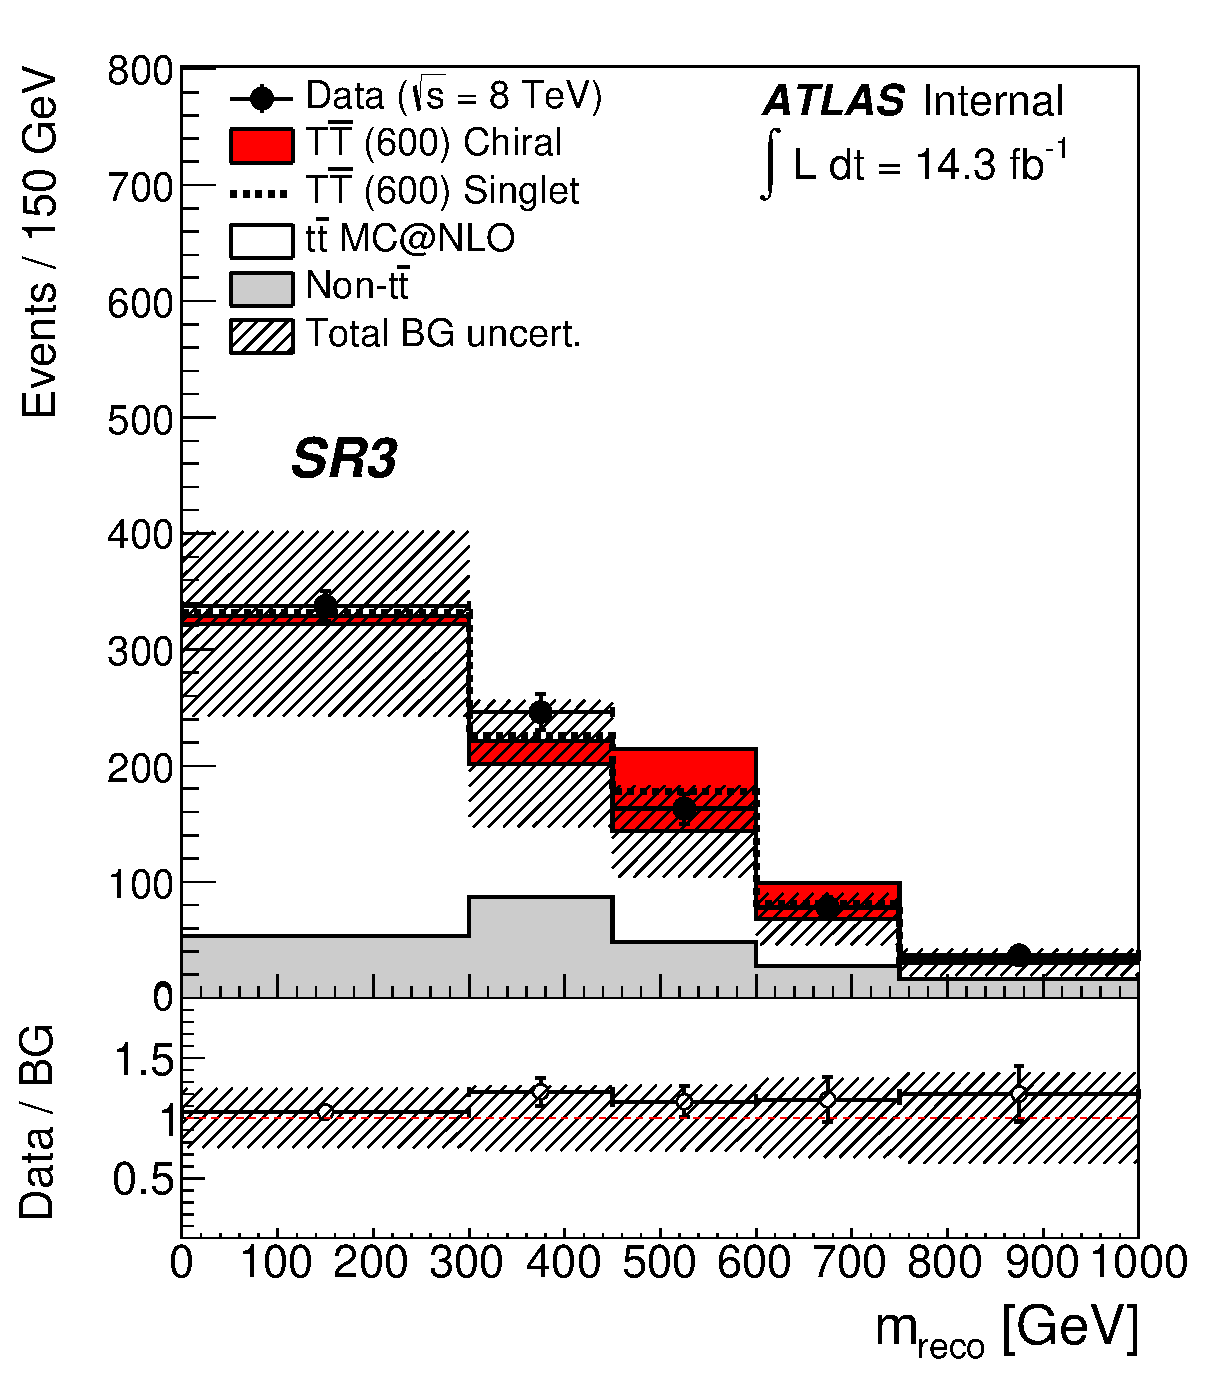
\includegraphics[width=0.37\textwidth]{wbx_analysis_14ifb/figures/THESIS_c6_cutflow/VLQAna_WbX_1W_MWb_4_ELEMUON_cutflow123_NOMINAL.eps}}
	\subfigure[]{\label{fig:mrecoSR4}
  	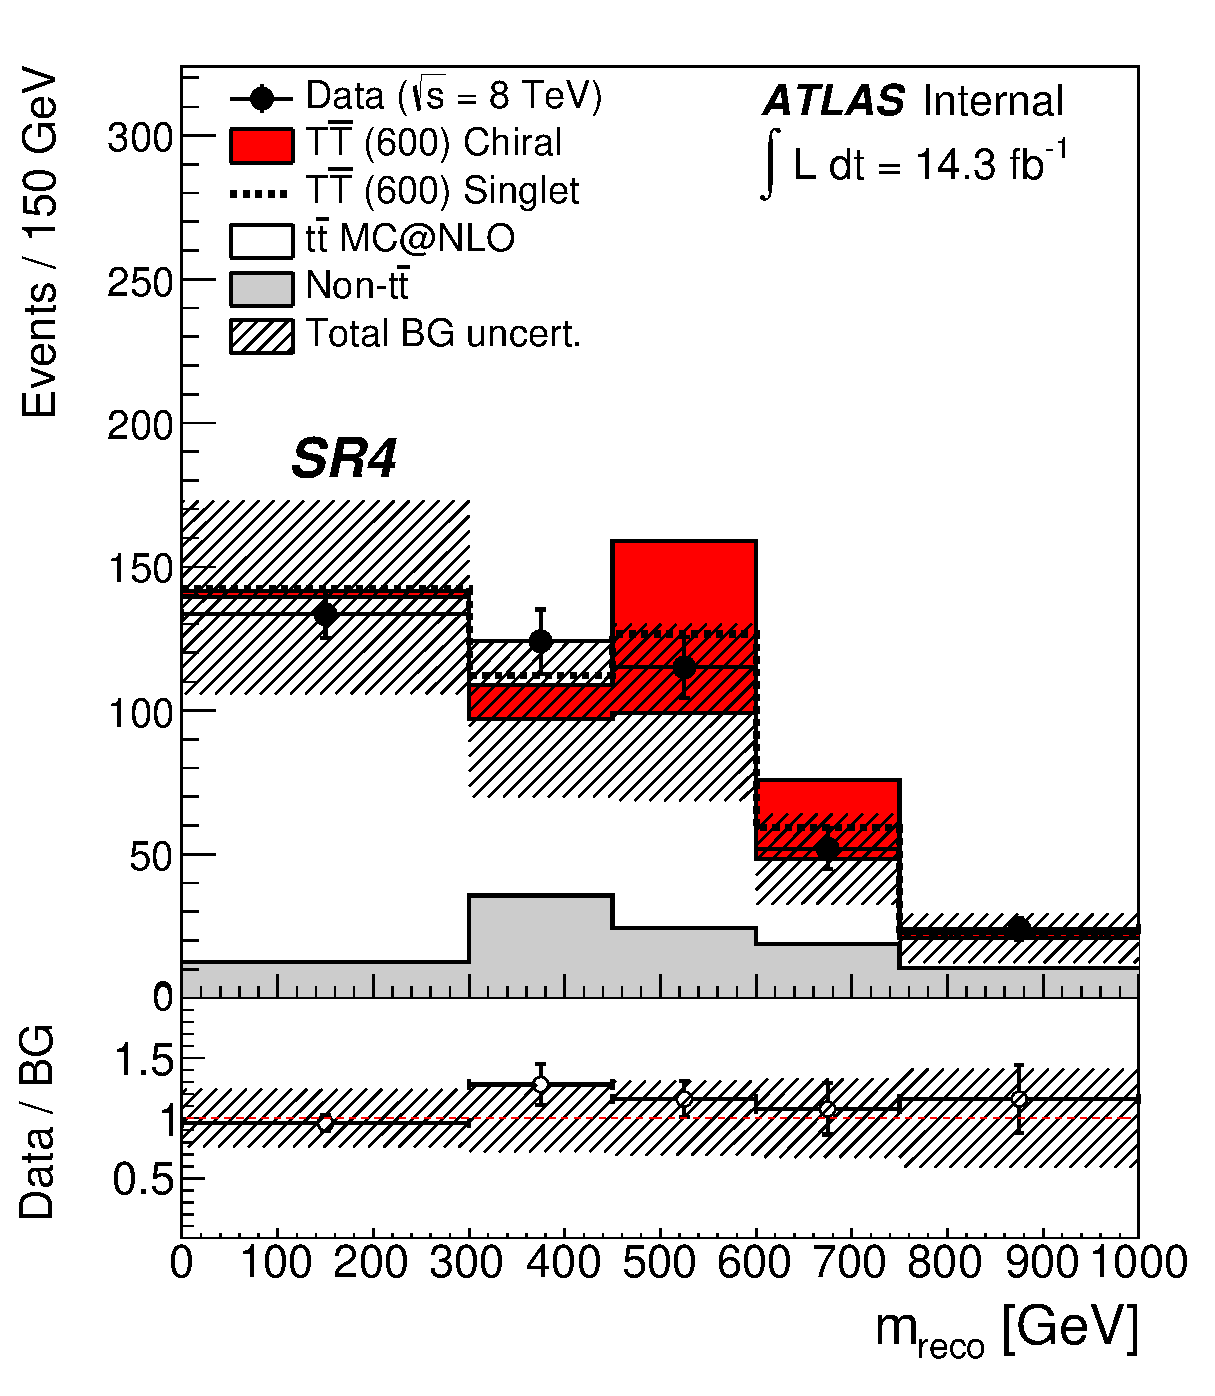
\includegraphics[width=0.37\textwidth]{wbx_analysis_14ifb/figures/THESIS_c6_cutflow/VLQAna_WbX_1W_MWb_4_ELEMUON_cutflow1234_NOMINAL.eps}}
	\subfigure[]{\label{fig:mrecoSR5}
  	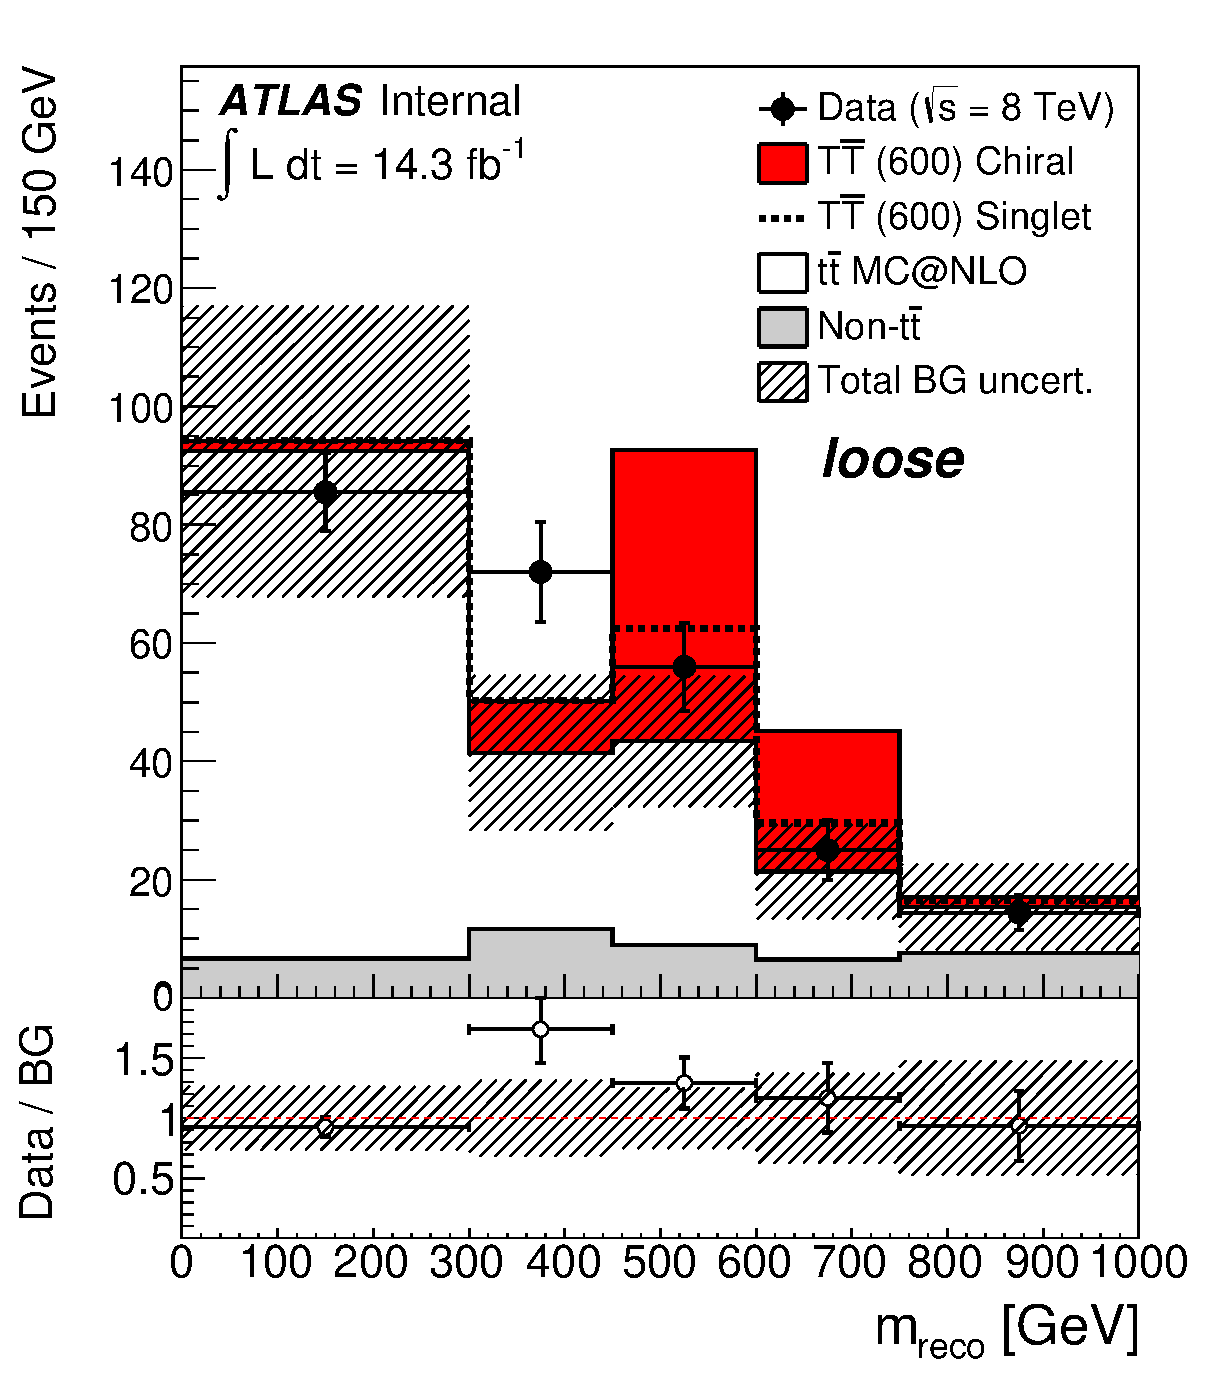
\includegraphics[width=0.4\textwidth]{wbx_analysis_14ifb/figures/THESIS_c6_cutflow/VLQAna_WbX_1W_MWb_4_ELEMUON_cutflow12345_NOMINAL.eps}}
	\subfigure[]{\label{fig:mrecoSR6}
  	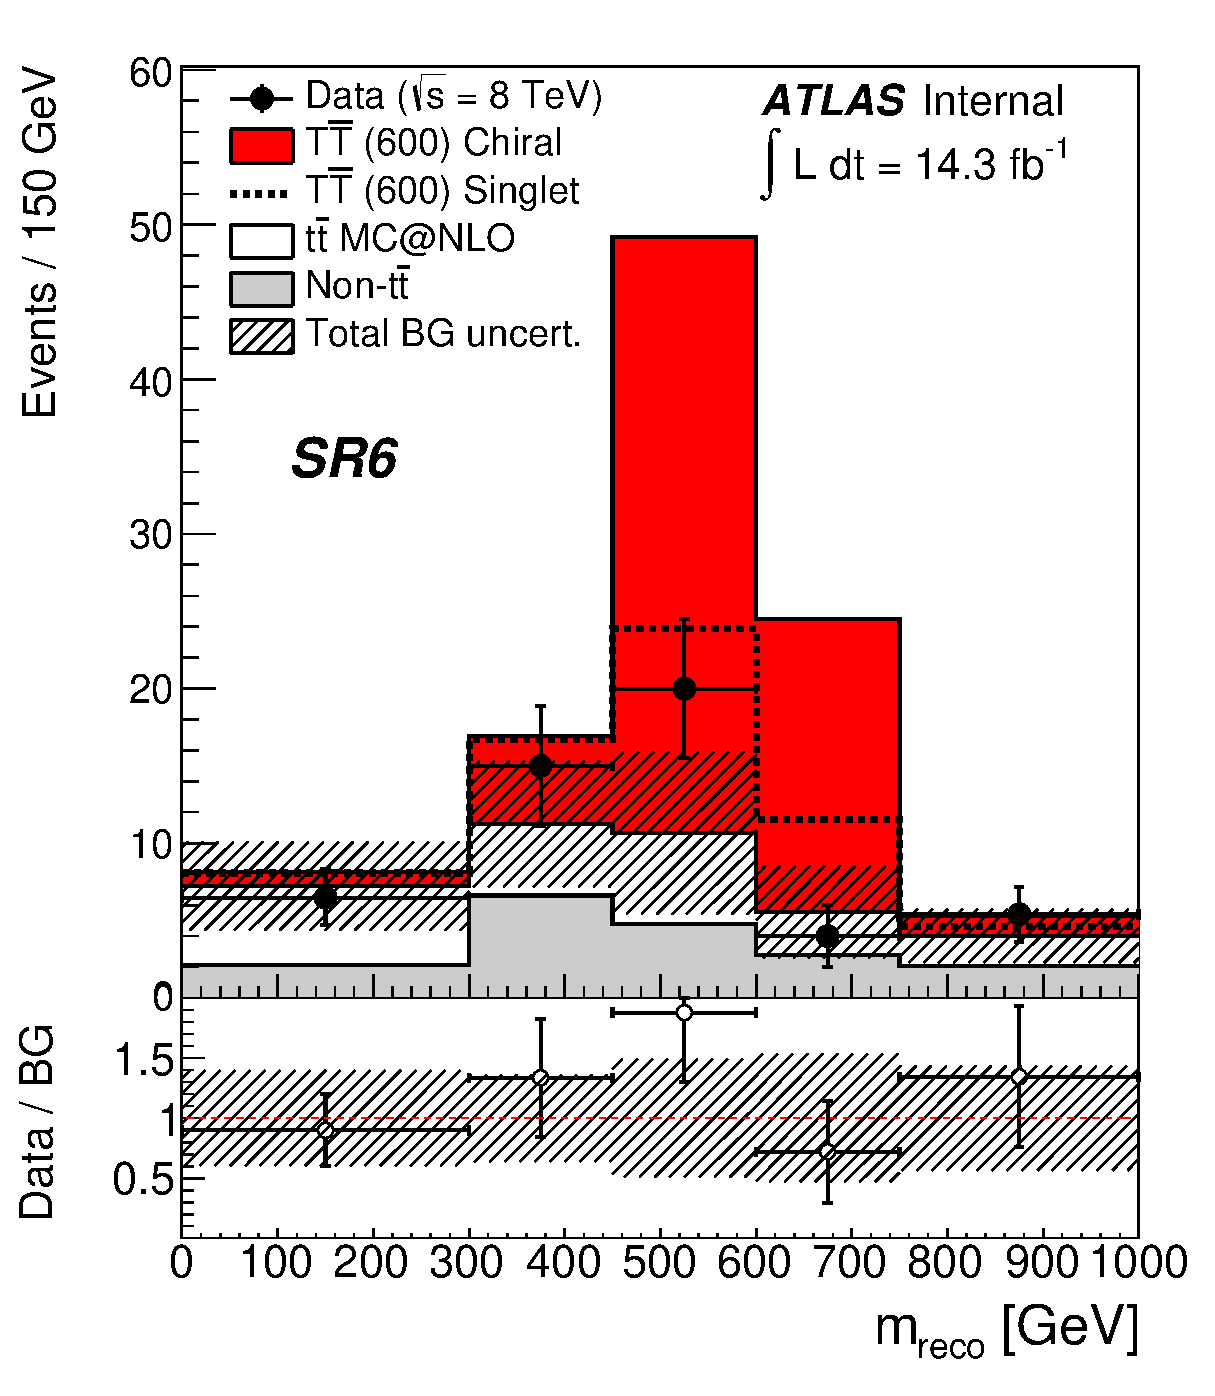
\includegraphics[width=0.4\textwidth]{wbx_analysis_14ifb/figures/THESIS_c6_cutflow/VLQAna_WbX_1W_MWb_4_ELEMUON_cutflow123456_NOMINAL.eps}}
	\subfigure[]{\label{fig:mrecoSR7}
  	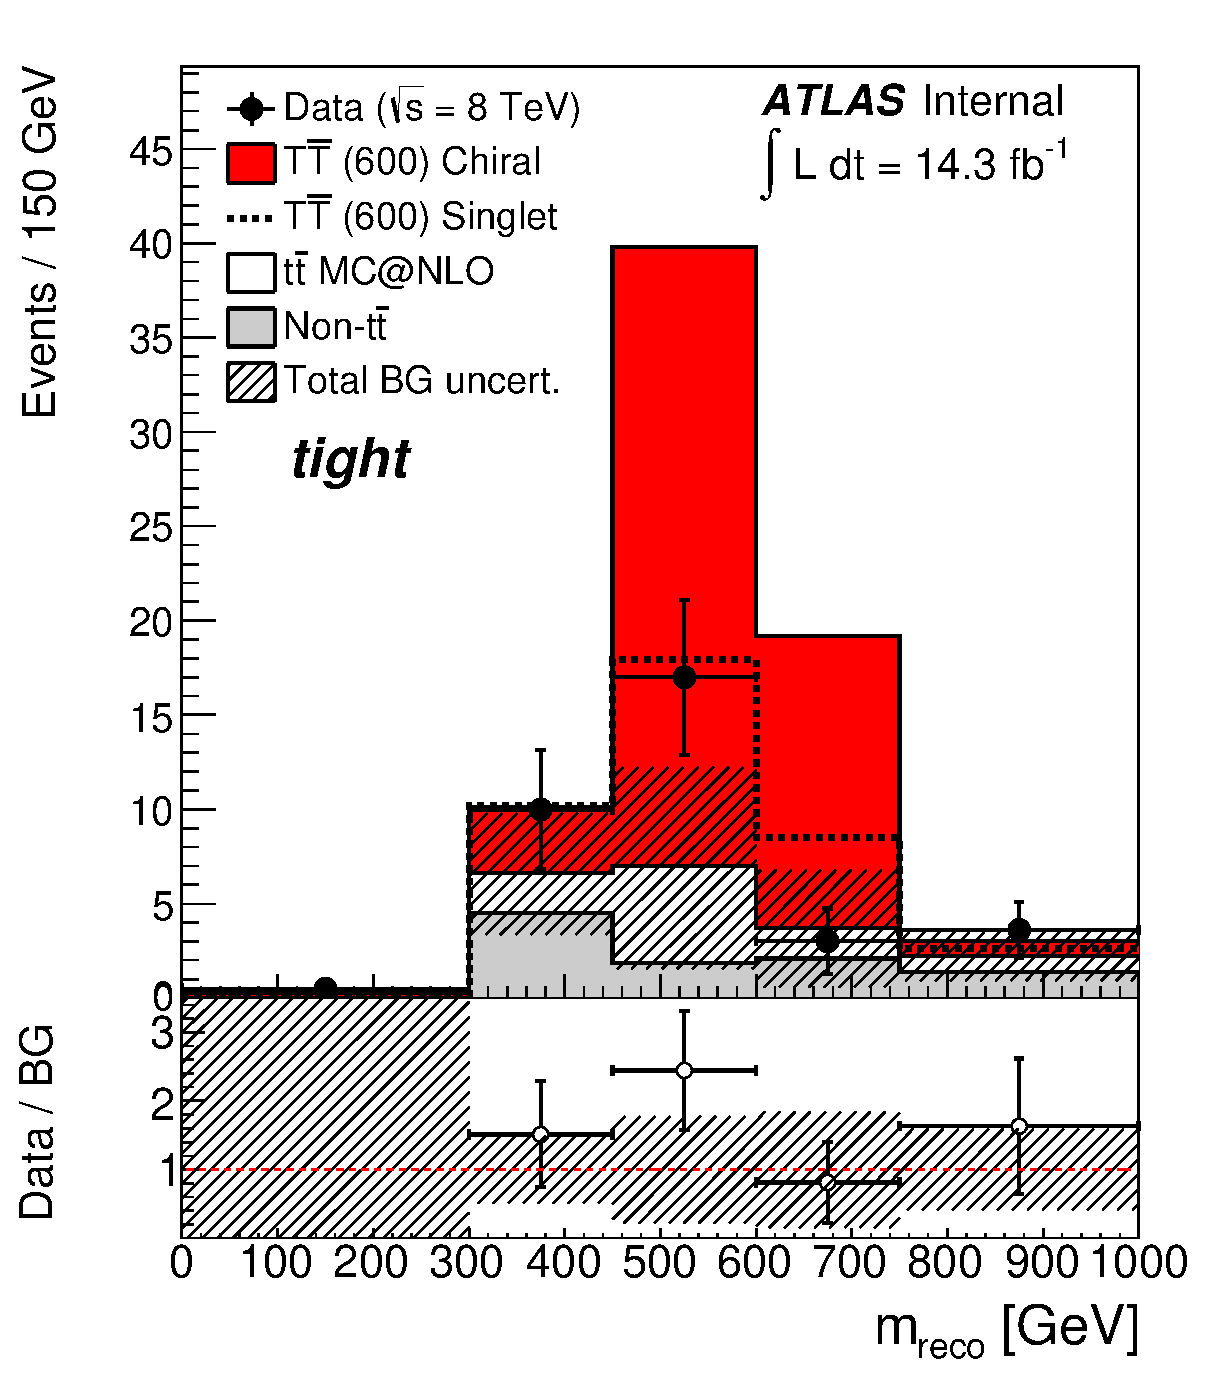
\includegraphics[width=0.4\textwidth]{wbx_analysis_14ifb/figures/THESIS_c6_cutflow/VLQAna_WbX_1W_MWb_4_ELEMUON_cutflow1234567_NOMINAL.eps}}
	\caption[bla]{Distribution of the reconstructed mass \mreco\ in the combined
        electron and muon channel for the various signal regions: (a) SR1, (b) SR2,
        (c) SR3, (d) SR4, (e) SR5 also known as \loose\ selection, (f) SR6
        and (e) SR7 also known as \tight\ selection.
        The data (solid black points) are compared to the background 
        prediction from Standard Model (stacked histograms). 
        The total uncertainty on the background estimation (see Section~\ref{sec:SystematicUncertainties} for details) is shown as a black hashed band.
        The expected contribution from a chiral fourth-generation 
        $\T$ quark with mass $m_{\T}=600\gev$ is also shown (red shaded histogram), 
        stacked on top of the Standard Model background. 
        The lower panel shows the ratio of data to Standard Model prediction. 
        The overflow has been added to the last bin.


\label{fig:mrecoSRs}}
\end{center}\end{figure}
\end{landscape}
